% !TeX program = lualatex
% Detailed version for master's seminar handout.
\documentclass[a4paper,10pt]{ltjsarticle}

\usepackage[top=20mm,bottom=22mm,left=18mm,right=18mm,columnsep=8mm]{geometry}
\usepackage{amsmath,amssymb}
\usepackage{graphicx}
\graphicspath{{figures/}}
\usepackage{booktabs}
\usepackage{multirow}
\usepackage{siunitx}
\usepackage{url}
\usepackage{caption}
\usepackage{subcaption}
\usepackage{xcolor}

\captionsetup{font=small,labelfont=bf}
\setlength{\parskip}{0.35em}
\setlength{\parindent}{1em}
\linespread{1.0}

\title{\vspace{-5mm}HISUIデータを用いたメタンプルーム検出における\\
Iterative Matched Filterと線状ノイズ除去の詳細検討}
\author{坂本優斗}
\date{}

\begin{document}
\twocolumn[
  \begin{@twocolumnfalse}
\maketitle

\begin{abstract}
Methane plume detection from hyperspectral satellite imagery is often performed using a matched filter (MF), which enhances spectral deviations consistent with methane absorption relative to a local background. In this study, we applied an iterative MF-like procedure to HISUI shortwave-infrared data and investigated line-shaped artifacts that appeared in the MF alpha image. The observed artifacts were not a single type of stripe: thin high-alpha lines produced false-positive pixels in the plume mask, while broader band-like offsets increased the dispersion of the alpha image. To address these effects, we estimated stripe directions from a larger scene, grouped pixels along the detected directions and their orthogonal directions, and subtracted line-group offsets inside each iteration of the MF procedure. We compared mean, median, and mode statistics for the thin-line cleanup while using median for the broad-band cleanup. For the 200-by-200 pixel region of interest, the cleanup reduced plume-mask pixels from 408 to 222--263 depending on the statistic. The mean statistic achieved the largest reduction in plume-mask pixels, whereas the median statistic achieved the lowest robust standard deviation. Spectral checks of selected pixels further suggested that line-artifact pixels and plume-candidate pixels have different residual spectra and per-band MF contributions. These results indicate that separating thin high-alpha artifacts from broader offset artifacts is useful for improving MF-based methane plume screening.
\end{abstract}

\vspace{1em}
  \end{@twocolumnfalse}
]

\section{はじめに}
メタンは二酸化炭素に次ぐ重要な温室効果ガスであり，局所的な排出源を検出し，その位置と規模を把握することは，排出削減や漏洩監視の観点から重要である．近年は，PRISMA，EMIT，GHGSat，MethaneSATなど，短波長赤外域を観測できる衛星・航空機センサを用いたメタン点源検出が進んでいる\cite{foote2020,pei2023,emit}．これらの手法では，メタン吸収が現れる波長帯のスペクトル情報を利用し，背景スペクトルからのメタンらしい偏差を画像上に可視化する．

Matched Filter（MF）は，そのようなメタン検出で広く使われるデータ駆動型の手法である\cite{mf}．MFは，各pixelの観測スペクトルを背景スペクトルと比較し，あらかじめ用意したメタン吸収テンプレートと整合する成分を強調する．その出力であるalpha画像は，メタン吸収らしさを表すスコア画像として解釈できるため，閾値処理によりplume maskを作成できる．一方で，MFは背景平均や背景共分散の推定に敏感であり，背景に含まれる地表スペクトルの不均一性，センサ由来の線状ノイズ，あるいは強いplume pixelの混入により，偽陽性を生じることがある．

本研究では，HISUIの短波長赤外域データに対してMFおよびIterative MFを適用したところ，メタンプルームとは考えにくい線状応答がalpha画像に現れた．特に，細い高alpha線はplume maskに直接残りやすく，太い帯状offsetはalpha画像全体のばらつきを増加させた．そこで本研究では，シーン全体から線状ノイズの傾きを推定し，対象ROI内でline groupごとのoffsetを差し引くdestripingをIterative MFの各iteration内に組み込む方法を検討した．本稿では，MFの構造，背景更新の意味，傾き検出，destriping処理，統計量比較，スペクトル確認の順に整理する．

\section{対象データと解析方針}
\subsection{HISUI短波長赤外データ}
解析には，HISUIの短波長赤外域スペクトルを用いた．現在の評価では，シーン全体から線状ノイズの傾きを推定し，その中の200$\times$200 pixelのROIを詳細解析対象とした．各pixelについて波長ごとの放射輝度スペクトルをCSV形式で扱い，メタン吸収テンプレートにはMODTRANに基づくCH$_4$参照スペクトルを用いた．主に\SIrange{2100}{2450}{nm}の波長範囲を使用した．この波長帯はメタン吸収が強く現れる一方，地表反射率やセンサノイズの影響も受けるため，背景推定の扱いが重要になる．

図\ref{fig:overview}に，シーン全体のMF alpha画像，解析対象ROI，ROI内のraw alpha画像，初期plume maskを示す．シーン全体のalpha画像には，画像の回転方向に沿うような細かい縞状構造が見られる．ROI内にも同じ傾きの高alpha線が残っており，初期plume maskでは左下付近の斜め線が偽陽性として抽出されている．このため，単にROI内だけでノイズを見積もるのではなく，より広いシーン全体から線方向を推定する方針を採った．

\begin{figure*}[t]
  \centering
  \begin{subfigure}{0.24\textwidth}
    \centering
    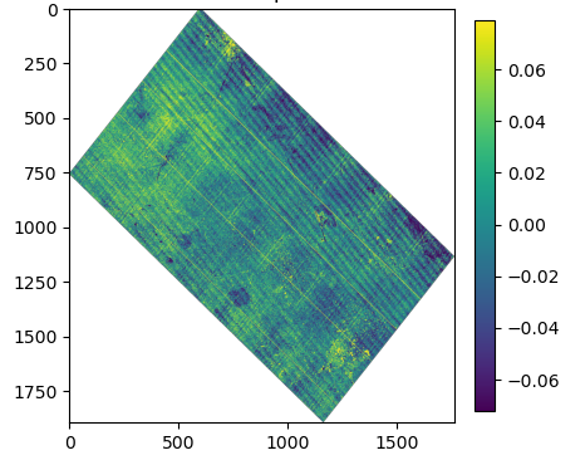
\includegraphics[width=\linewidth]{allmap_MF.png}
    \caption{Full-scene MF alpha}
  \end{subfigure}
  \hfill
  \begin{subfigure}{0.24\textwidth}
    \centering
    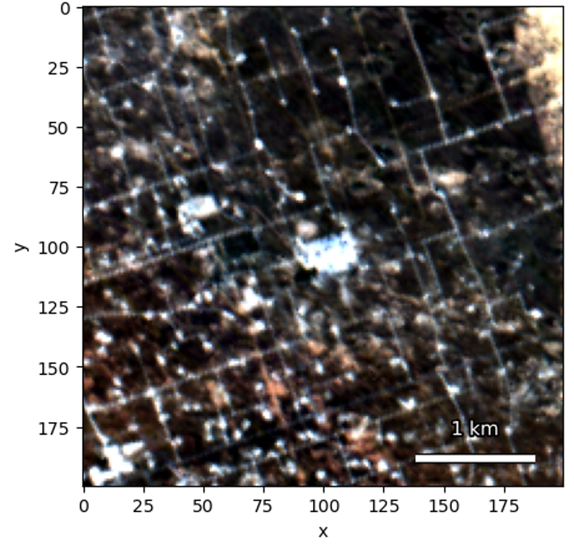
\includegraphics[width=\linewidth]{roi_preview.png}
    \caption{ROI preview}
  \end{subfigure}
  \hfill
  \begin{subfigure}{0.24\textwidth}
    \centering
    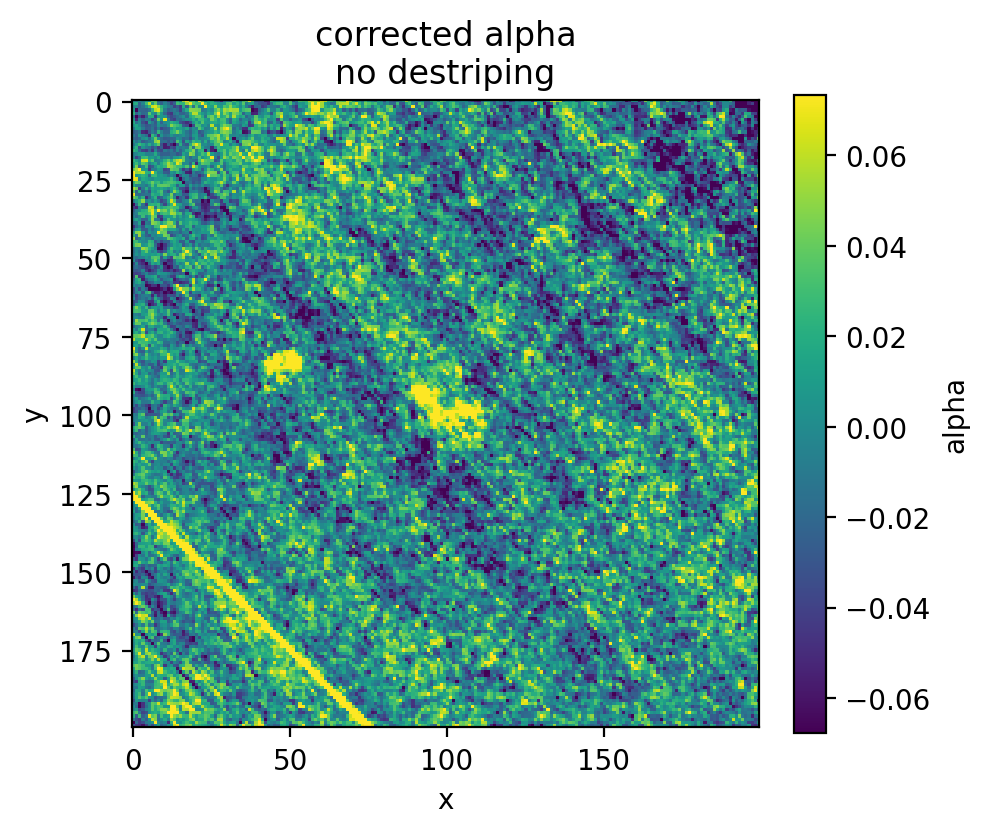
\includegraphics[width=\linewidth]{raw_alpha.png}
    \caption{Raw alpha}
  \end{subfigure}
  \hfill
  \begin{subfigure}{0.24\textwidth}
    \centering
    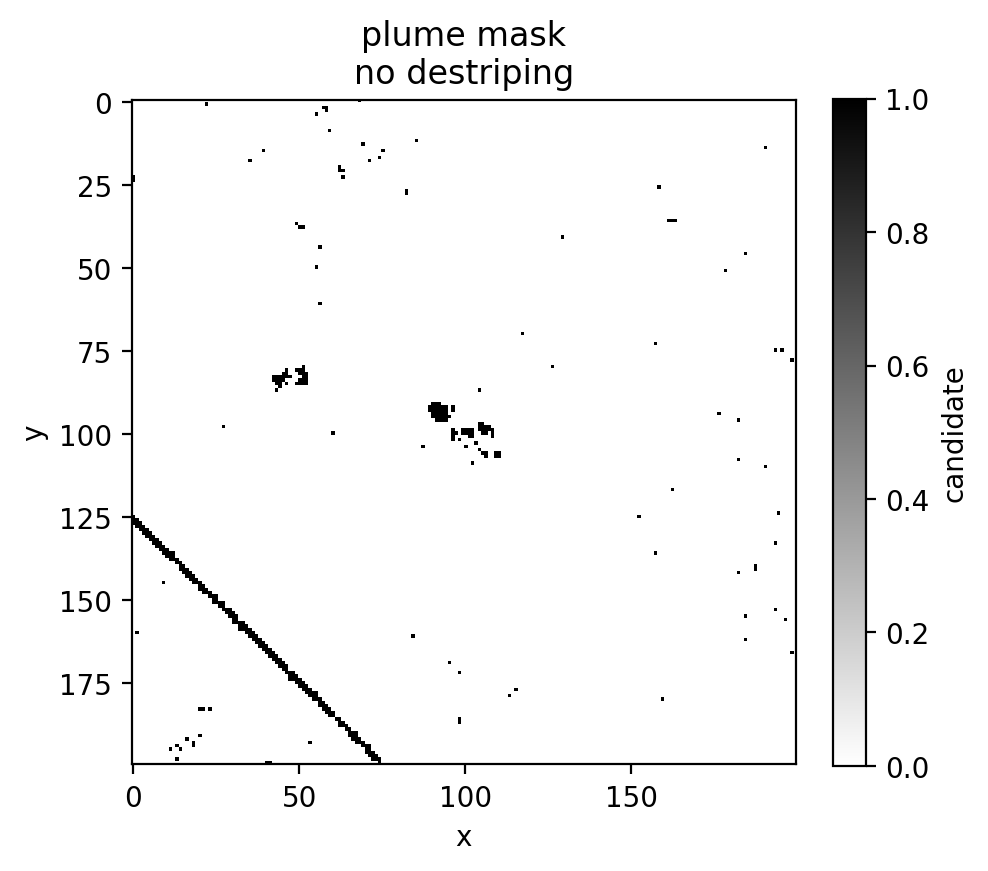
\includegraphics[width=\linewidth]{initial_plume_mask.png}
    \caption{Initial plume mask}
  \end{subfigure}
  \caption{Overview of the full-scene MF result and analyzed ROI. The full-scene alpha image was used to estimate line directions, while the 200-by-200 ROI was used for detailed destriping and plume-mask evaluation.}
  \label{fig:overview}
\end{figure*}

\subsection{解析の基本方針}
本研究の目的は，メタンplume候補を過度に消さずに，線状偽陽性を抑制することである．そのため，本稿では次の二つの評価量を用いた．第一に，plume mask上の候補pixel数である．これは，線状偽陽性がどれだけmaskに残っているかを示す直接的な指標である．第二に，alpha画像全体のrobust standard deviation（RStd）である．これは，補正後alpha画像のばらつきを表し，太い帯状offsetが抑えられているかを見る指標である．

ただし，候補pixel数を減らすことだけを目的にすると，実際のplume候補まで削る可能性がある．逆に，RStdだけを小さくすることを目的にすると，plume mask上の細線が残る可能性がある．したがって，本研究では二つの指標を同時に見ながら，補正結果を評価した．

\section{Matched Filterの構造}
\subsection{MF alphaの意味}
MFは，各pixelの観測スペクトルにメタン吸収テンプレートがどの程度含まれるかを，背景との差として評価する手法である．各pixelの観測スペクトルを$\mathbf{x}_i$，背景平均を$\boldsymbol{\mu}$，背景共分散を$\mathbf{C}$，メタン吸収テンプレートを$\mathbf{t}$とすると，MF alphaは
\begin{equation}
  \alpha_i =
  \frac{(\mathbf{x}_i-\boldsymbol{\mu})^\top \mathbf{C}^{-1}\mathbf{t}}
       {\mathbf{t}^\top \mathbf{C}^{-1}\mathbf{t}}
  \label{eq:mf}
\end{equation}
で表される．分子は，背景平均からの差分$(\mathbf{x}_i-\boldsymbol{\mu})$を，背景共分散で重み付けした上でメタンテンプレート方向に射影する量である．分母はテンプレートの正規化項であり，alpha値のスケールを揃える役割を持つ．

ここで重要なのは，共分散$\mathbf{C}$が単なる分散ではなく，波長間の相関も含むことである．ある波長で明るい地表は，別の波長でも明るい場合が多い．そのような背景の自然な変動は，メタン吸収とは区別されるべきである．MFでは$\mathbf{C}^{-1}$により，背景でよく起こる変動方向の重みを下げ，背景では起こりにくくメタンテンプレートに近い変動を強調する．

\subsection{背景推定と偽陽性}
MFの性能は，背景平均$\boldsymbol{\mu}$と背景共分散$\mathbf{C}$の推定に強く依存する．背景集合にメタンplume pixelが含まれると，メタン吸収を持つスペクトルが背景として扱われ，alpha値が過小評価される可能性がある．一方，地表の不均一性やセンサ由来の線状応答が背景統計に混入すると，メタン吸収とは異なる構造がalpha画像に現れることがある．

本研究で問題となった線状応答は，メタン吸収テンプレートそのものだけで説明するには不自然であった．例えば，左下の斜め線は幾何学的に非常に細く，地物やplumeの拡散形状としては解釈しにくい．また，シーン全体に広がる帯状offsetは，局所的なメタン排出ではなく，背景推定やセンサ幾何に由来する系統誤差として扱う方が自然である．

\section{Iterative MFと背景mask更新}
\subsection{反復処理の考え方}
Iterative MFでは，初期背景からMF alphaを計算し，高alpha pixelをplume候補として背景から除外した後，再度背景統計量を推定する．この処理を繰り返すことで，強いplume候補が背景平均や共分散に混入する影響を抑える．本研究では，Pei et al.のIterative Lognormal Matched Filter（ILMF）\cite{pei2023}の考え方を参考に，背景maskを反復更新する構成を用いた．ただし，本研究の主眼は濃度定量ではなく，MF alpha画像に現れる線状偽陽性の除去である．

各iterationでは，まず現在の背景maskに基づいて$\boldsymbol{\mu}$と$\mathbf{C}$を推定し，式(\ref{eq:mf})によりalpha画像を計算する．次に，alpha画像に対して線状ノイズ除去を行う．その後，補正後alpha画像からrobust thresholdを用いて新しいplume maskを作成し，背景maskを更新する．この順序により，線状偽陽性が次の背景推定から過度に除外されることを防ぎつつ，実plume候補は背景から除くことを狙った．

\subsection{robust threshold}
plume maskの閾値には，alpha画像のmedianとmedian absolute deviation（MAD）に基づくrobust standard deviationを用いた．alpha画像を$\alpha$とすると，
\begin{equation}
  \sigma_{\mathrm{robust}} =
  1.4826 \ \mathrm{median}\left(|\alpha - \mathrm{median}(\alpha)|\right)
  \label{eq:rstd}
\end{equation}
であり，閾値は
\begin{equation}
  T = \mathrm{median}(\alpha) + k\sigma_{\mathrm{robust}}
  \label{eq:threshold}
\end{equation}
とした．ここで$k$は本解析では主に3を用いた．medianとMADを使う理由は，高alpha pixelや線状外れ値の影響を平均と標準偏差より受けにくいためである．

\section{線状ノイズの観察}
\subsection{細い高alpha線と太い帯状offset}
Iterative MFのalpha画像には，主に二種類の不自然な線状応答が確認された．第一は，$y=x$に近い向きを持つ細い高alpha線である．これは局所的にalpha値が高く，plume mask上では細い線として抽出されやすい．第二は，より太い帯状のalpha offsetである．これはmask上の細線として目立つだけでなく，alpha画像全体のばらつきを増加させる．

この二種類の線は，同じ「stripe」として一括処理すると扱いにくい．細い高alpha線は，高alpha pixelの集中を見れば検出しやすいが，太い帯状offsetは必ずしも高alpha pixelだけとして現れるわけではない．逆に，太い帯状offsetは画像全体のばらつき低下を基準に検出できるが，細い線を同じ基準で評価すると局所的な偽陽性を見逃す可能性がある．そのため，本研究では細い線と太い帯状offsetを分けて検出し，それぞれに適した評価量を用いた．

\subsection{destripingの先行例との関係}
光学衛星画像では，pushbroom型センサの走査方向に沿って系統誤差が現れることがある．Koga and Iwasaki\cite{koga2011}は，ASTERステレオ画像から得られるDEM差分に対して，センサ幾何上のline/column番号を利用し，走査線方向の誤差をdestripingすることで地形変化計測精度を改善した．本研究の対象はDEMではなくMF alpha画像であるが，「センサ幾何や画像上の線方向に沿って系統的なoffsetを推定し，差し引く」という点では同じ考え方に基づいている．

\section{シーン全体を用いた傾き検出}
\subsection{line groupへの分割}
200$\times$200 pixelのROIだけでは，線状ノイズの傾きを安定に推定しにくい．そこで，より広いシーン全体のMF結果を用いて線方向を推定した．正の傾き$a$を仮定し，各pixelを
\begin{equation}
  b = y - ax
  \label{eq:bgroup}
\end{equation}
によりline groupに分ける．同じ$b$を持つpixelは，傾き$a$の直線上に並ぶ．直交方向については，傾き$a_\perp=-1/a$を考え，
\begin{equation}
  b_\perp = y - a_\perp x
  \label{eq:bperp}
\end{equation}
でgroup化した．実装上は，連続値である$b$を一定bin幅で丸め，同じbinに属するpixelを一つのline groupとして扱った．

図\ref{fig:slope_overlay}に，検出された線方向とその直交方向をシーン全体に重ねた例を示す．今回使用した傾きは，細い線が$+0.9793$およびその直交方向$-1.0212$，太い線が$+1.2572$およびその直交方向$-0.7954$である．

\begin{figure*}[t]
  \centering
  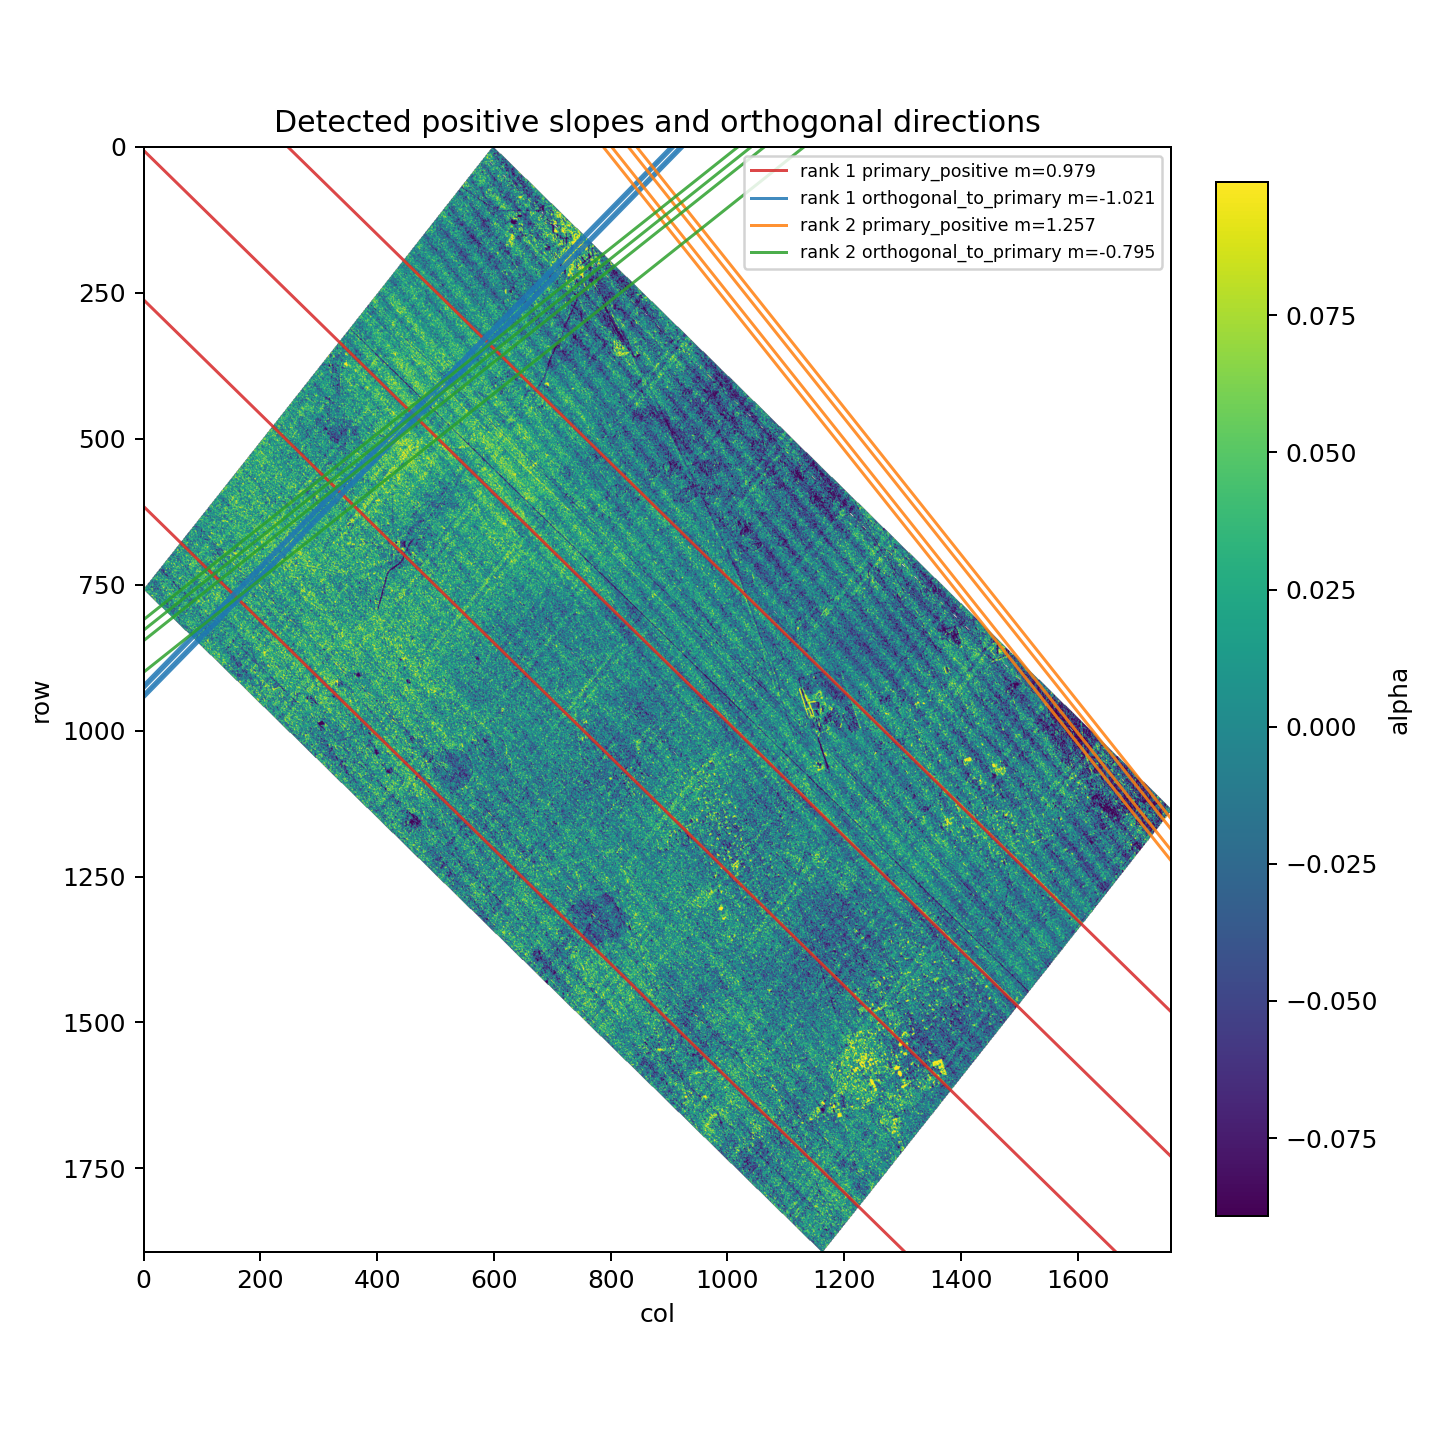
\includegraphics[width=0.78\textwidth]{detected_slope_overlay.png}
  \caption{Detected line directions overlaid on the full-scene MF alpha image. The two primary positive-slope directions and their orthogonal directions were used for the subsequent line-group destriping.}
  \label{fig:slope_overlay}
\end{figure*}

\subsection{細い線の検出スコア}
細い高alpha線では，高alpha pixelが少数のline groupに集中する．そこで，候補傾きごとにline groupを作り，各groupに含まれる高alpha pixelの集中度を評価した．高alpha pixelは，alpha画像のrobust thresholdを超えたpixelとして定義した．線が存在する傾きでは，あるgroupに高alpha pixelが集中するため，スコア曲線に鋭いピークが現れる．

図\ref{fig:slope_scores}(a)に，細い線検出のスコア曲線を示す．raw scoreには大きなピークがあり，rolling median trendから大きく突出している．本研究では，単純なスコア最大値ではなく，rolling medianにより角度方向の背景トレンドを推定し，そのトレンドから突出する局所ピークを選択した．これにより，スコアが角度に対して単調増加する場合でも，孤立した線方向を選びやすくした．

\subsection{太い帯状offsetの検出スコア}
太い帯状offsetは，必ずしも高alpha pixelの集中として現れない．そのため，候補傾きごとにline group補正を仮に行い，補正前後でalpha画像のrobust standard deviationがどれだけ低下するかを評価した．これは，線方向に沿って共通のoffsetが存在するなら，その方向でgroupごとの代表値を差し引くと画像全体のばらつきが小さくなる，という考え方である．

図\ref{fig:slope_scores}(b)に，太い帯状offset検出のスコア曲線を示す．細い線検出とはスコアの意味が異なるが，同様にrolling median trendから突出する局所ピークを選択した．このように，細い線と太い帯状offsetで検出基準を分けることにより，plume mask上の偽陽性とalpha画像全体のばらつきの両方に対応できる．

\begin{figure*}[t]
  \centering
  \begin{subfigure}{0.48\textwidth}
    \centering
    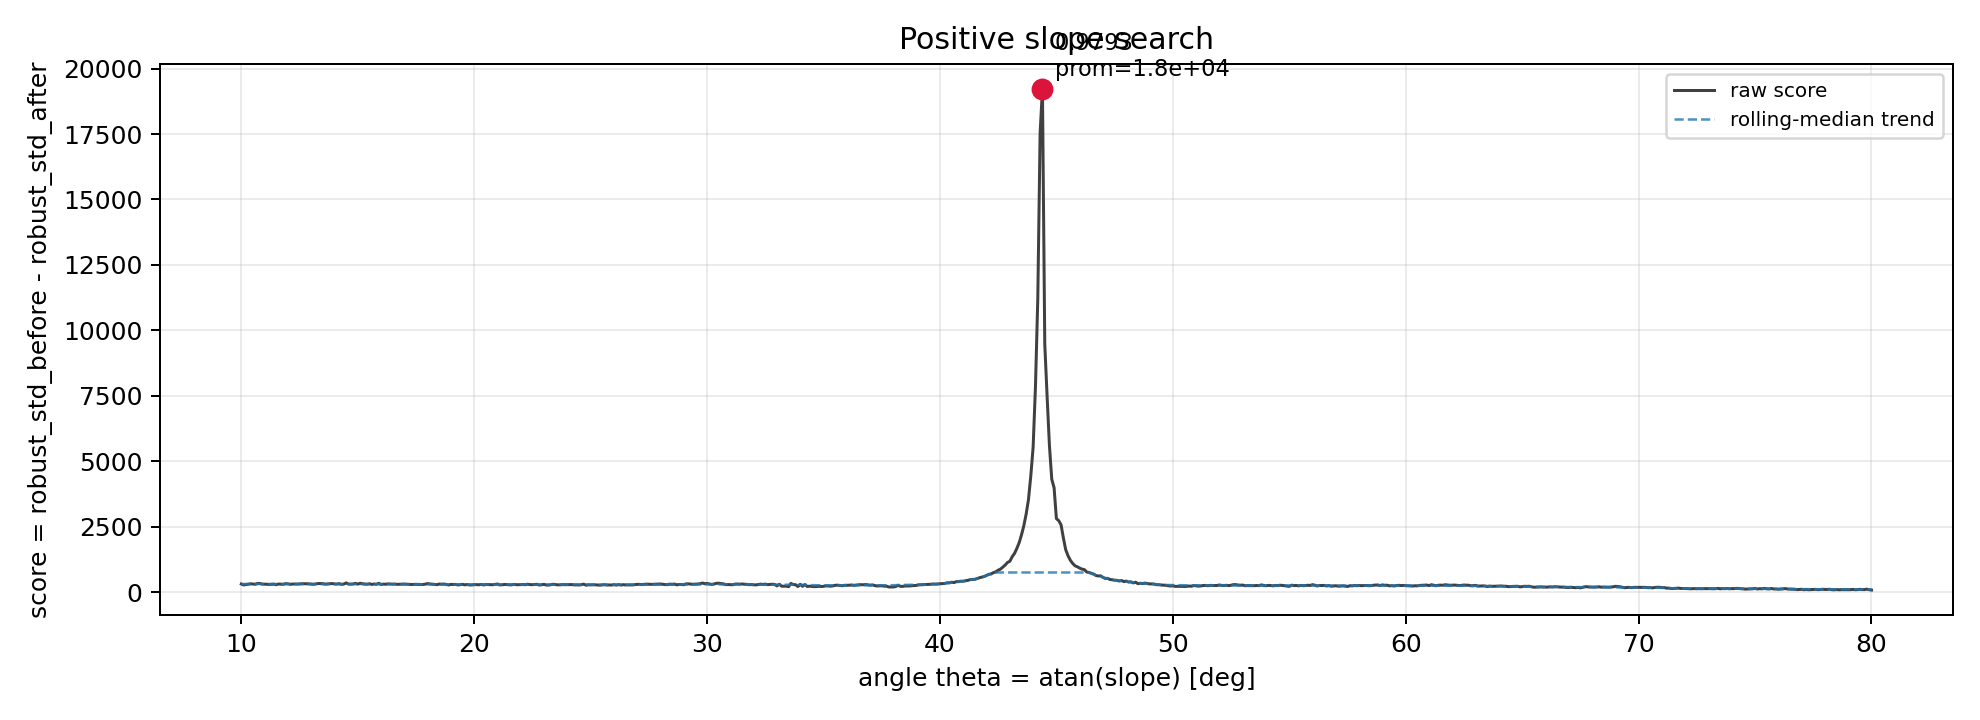
\includegraphics[width=\linewidth]{thin_slope_score_curve.png}
    \caption{Thin high-alpha line}
  \end{subfigure}
  \hfill
  \begin{subfigure}{0.48\textwidth}
    \centering
    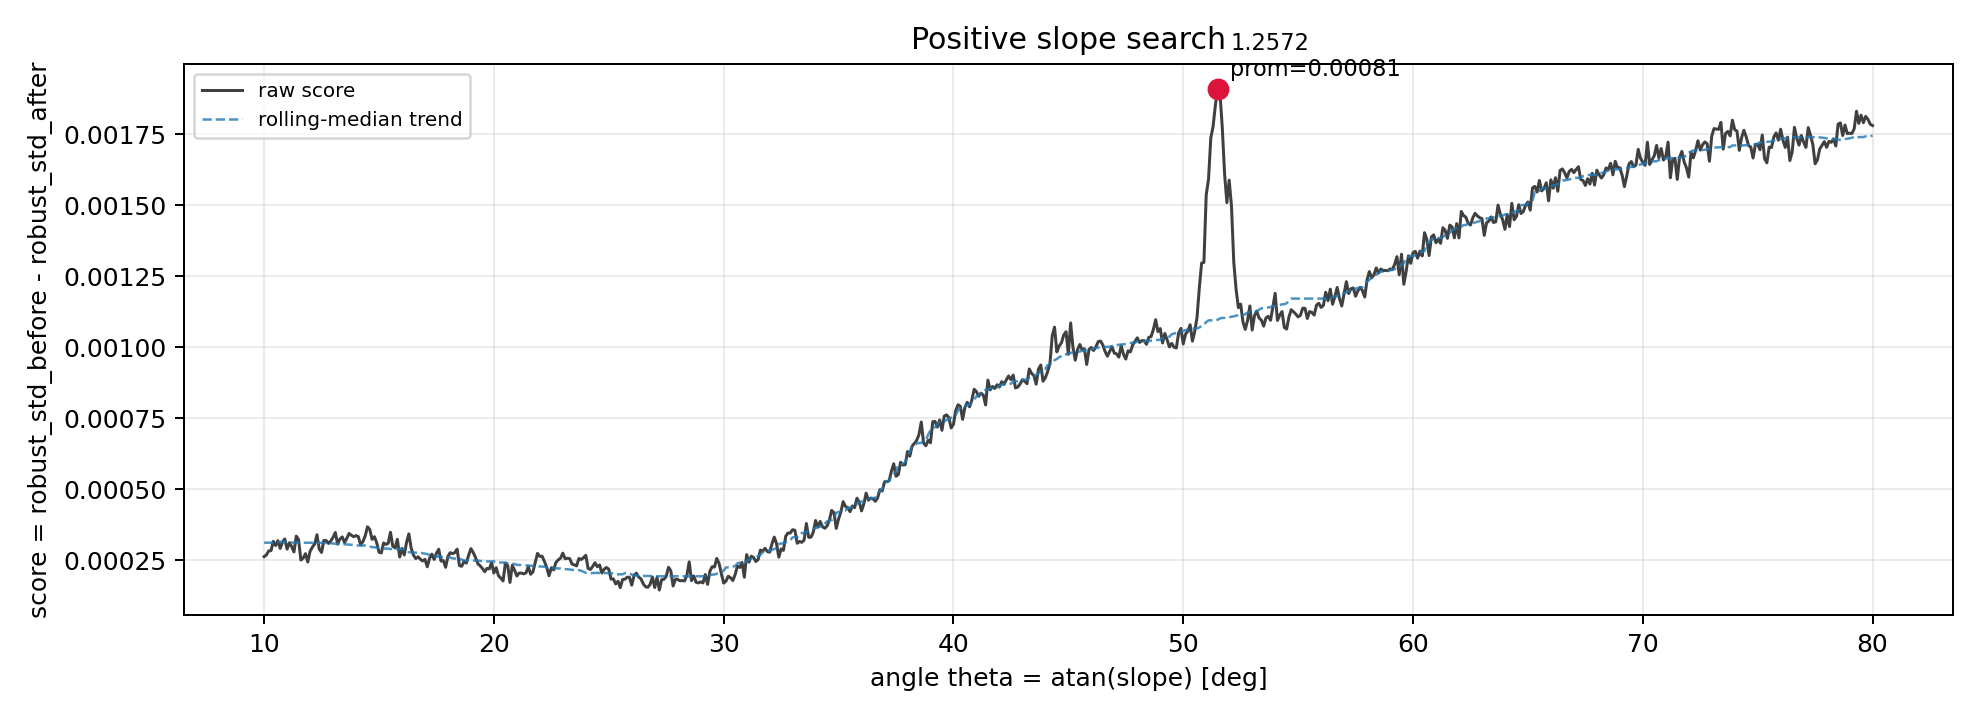
\includegraphics[width=\linewidth]{broad_slope_score_curve.png}
    \caption{Broad-band offset}
  \end{subfigure}
  \caption{Slope-search score curves. The thin-line score emphasizes concentration of high-alpha pixels, whereas the broad-offset score evaluates the robust-standard-deviation reduction after trial correction.}
  \label{fig:slope_scores}
\end{figure*}

\section{line groupに基づくdestriping}
\subsection{offset推定}
検出された線方向に対して，各pixelをline groupに分け，groupごとのalpha代表値から線状offsetを推定した．あるline group $b$の代表値を$s_b$，画像全体の代表値を$s_0$とすると，そのgroupの補正量は
\begin{equation}
  \Delta_b = s_b - s_0
  \label{eq:offset}
\end{equation}
である．該当line groupに属するpixelから$\Delta_b$を差し引くことで，group単位のoffsetを除去する．これは，alpha画像を線方向に沿った低次元の系列に集約し，その系列のずれを画像から引く処理と解釈できる．

代表値$s_b$には，mean，median，modeを比較した．meanは高alpha線を積極的に反映しやすく，細い線の補正量を大きく見積もりやすい．medianは外れ値に強く，太い帯状offsetのような緩やかなずれに対して安定である．modeは頻度の高い値を代表値とするが，連続値のalpha画像ではbinningや分布形状に敏感であり，中央値が大きくずれる場合があった．

\subsection{細い線と太い線で異なる処理}
細い高alpha線の補正では，高alpha線そのものをoffset推定に含める必要があるため，標準では高alpha pixelの除外を行わない．もし高alpha pixelを除外すると，除去したい線そのものが代表値推定から消え，補正量が小さくなる可能性がある．bin幅は2 pixel程度とし，細い線を局所的に捉えるようにした．

一方，太い帯状offsetでは，実plume候補がoffset推定に混入すると，plume信号まで差し引く危険がある．そこで，太い帯状offsetの補正ではrobust thresholdに基づく高alpha除外を用いた．また，bin幅は18 pixel程度とし，細かい線ではなく幅のある背景offsetを推定するようにした．このように，細い線と太い帯状offsetでは，代表値推定に含めるpixelとbin幅を変えた．

\subsection{Iterative MF内での補正順序}
本研究では，各iterationで次の順序を用いた．まず背景maskからMF alphaを計算する．次に，細い高alpha線を補正する．その後，太い帯状offsetを補正する．最後に，補正後alpha画像からrobust thresholdによりplume maskを作成し，次のiterationの背景maskを更新する．

この順序の意図は，plume maskに直接残りやすい細い線を先に抑え，その後に画像全体のばらつきを増やす太いoffsetを抑えることである．細い線を後に回すと，太いoffset補正の代表値推定に高alpha線が混入し，太いoffsetの推定が不安定になる可能性がある．一方，太いoffsetを補正しないままmaskを更新すると，背景maskの選択が線状offsetに影響される可能性がある．

\section{補正結果}
\subsection{代表例}
図\ref{fig:destripe_result}に，thin-line cleanupにmean，broad-band cleanupにmedianを用いた代表例を示す．raw alphaでは左下から右上に向かう細い高alpha線が見える．推定stripeには，細い線と広い帯状offsetの両方が含まれている．補正後alphaでは細い線状応答が弱まり，plume mask上でも左下の線状偽陽性が抑制されている．

\begin{figure*}[t]
  \centering
  \begin{subfigure}{0.24\textwidth}
    \centering
    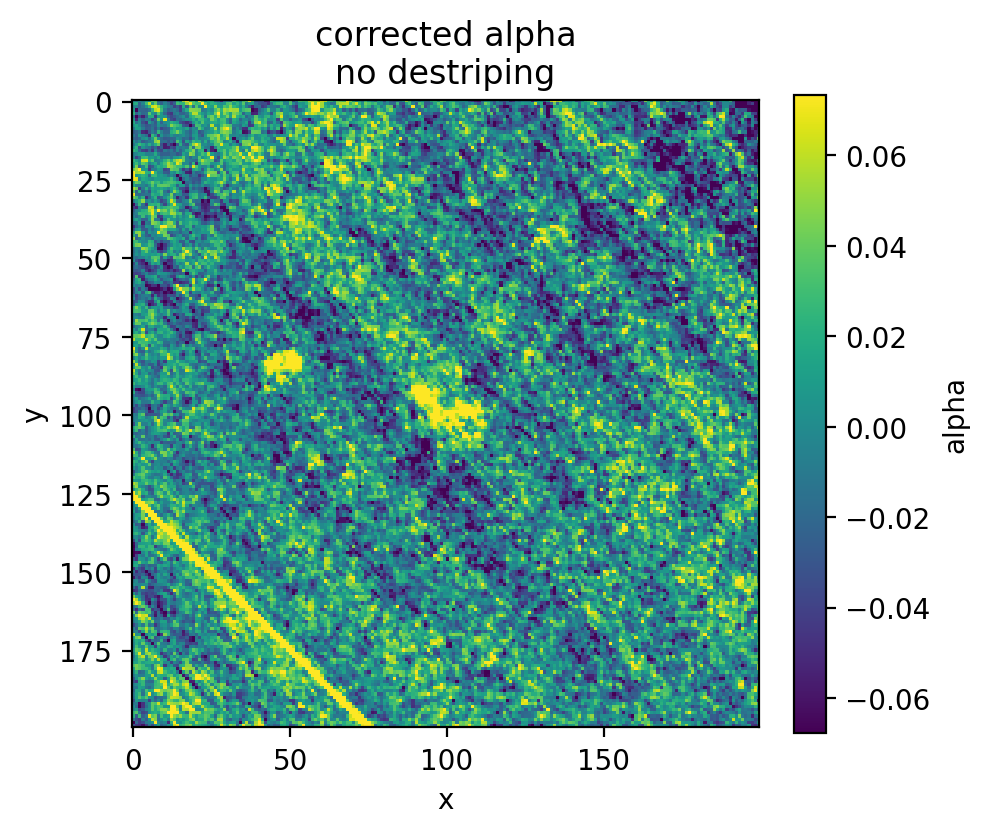
\includegraphics[width=\linewidth]{raw_alpha.png}
    \caption{Raw alpha}
  \end{subfigure}
  \hfill
  \begin{subfigure}{0.24\textwidth}
    \centering
    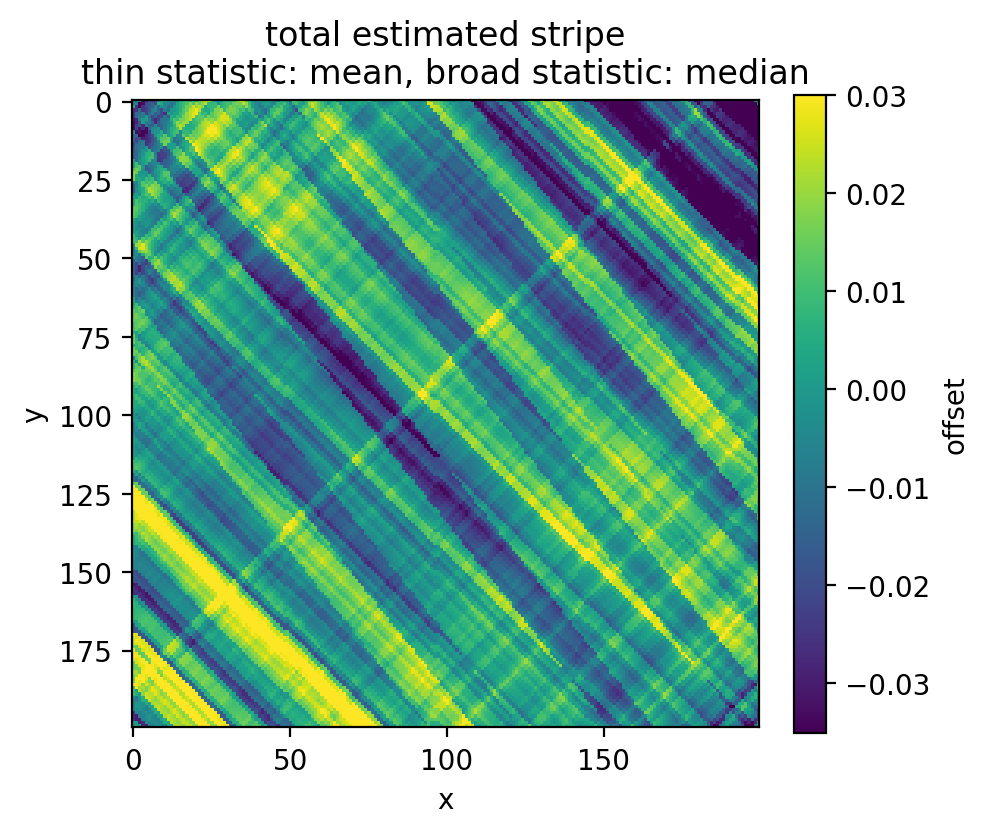
\includegraphics[width=\linewidth]{mean_detected_stripe.png}
    \caption{Estimated stripe}
  \end{subfigure}
  \hfill
  \begin{subfigure}{0.24\textwidth}
    \centering
    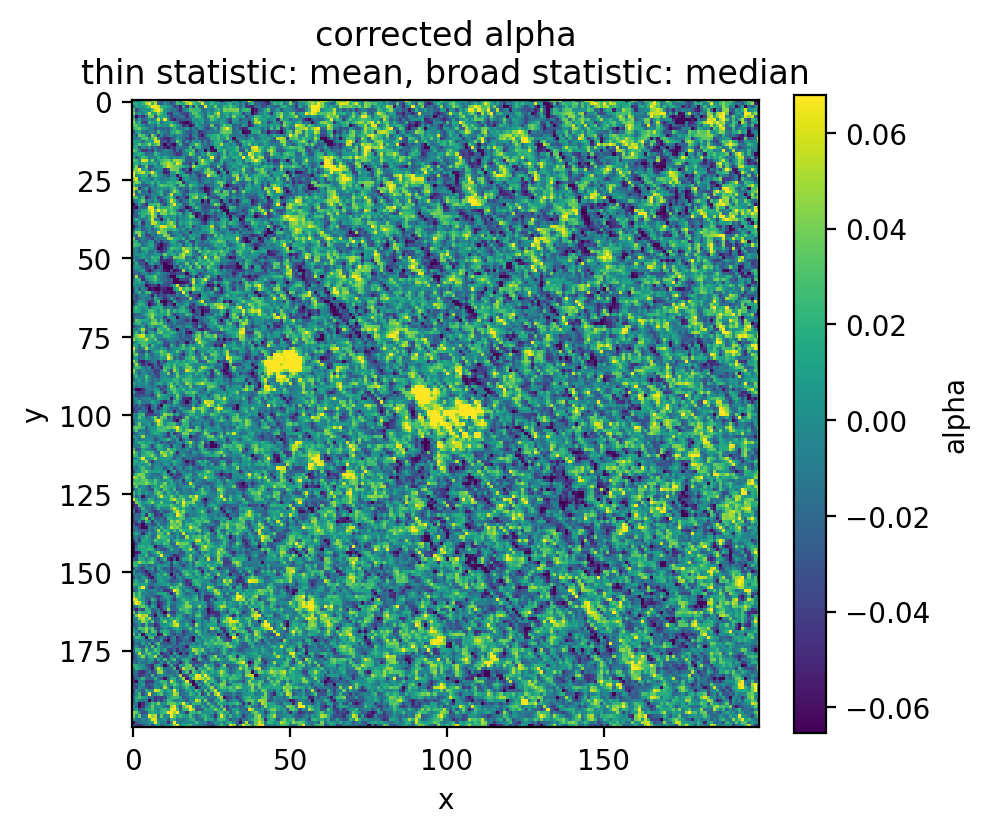
\includegraphics[width=\linewidth]{mean_corrected_alpha.png}
    \caption{Corrected alpha}
  \end{subfigure}
  \hfill
  \begin{subfigure}{0.24\textwidth}
    \centering
    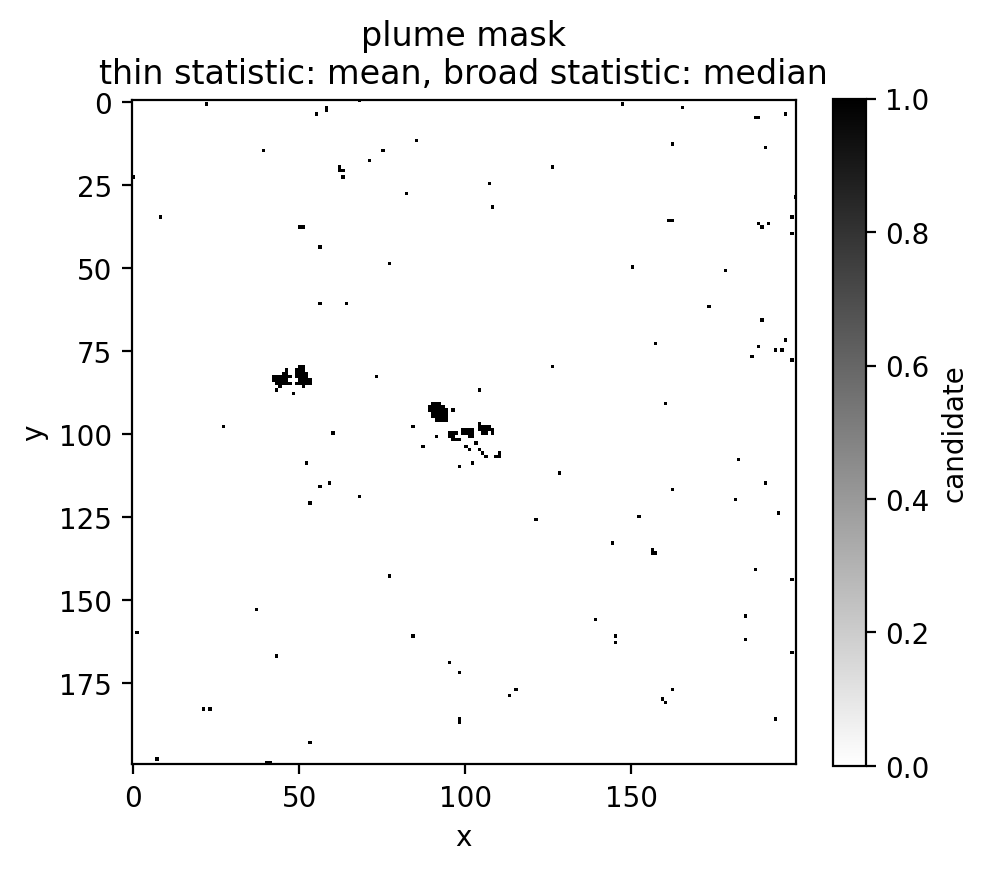
\includegraphics[width=\linewidth]{mean_plume.png}
    \caption{Plume mask}
  \end{subfigure}
  \caption{Example destriping result using mean for the thin-line cleanup and median for the broad-band cleanup. The estimated stripe image contains both thin high-alpha-line correction and broad-band offset correction.}
  \label{fig:destripe_result}
\end{figure*}

\subsection{統計量ごとのalpha画像比較}
図\ref{fig:alpha_comparison}に，baseline，mean，median，modeの補正後alpha画像を示す．baselineでは左下の斜め線が明瞭である．meanではこの細い線が強く抑えられているが，画像全体の細かなテクスチャも変化している．medianでは線状偽陽性の抑制はmeanより弱いが，画像全体のばらつきは最も低くなった．modeではplume候補数は減少したものの，alpha分布の代表値がずれやすく，安定性に課題が見られた．

\begin{figure*}[t]
  \centering
  \begin{subfigure}{0.24\textwidth}
    \centering
    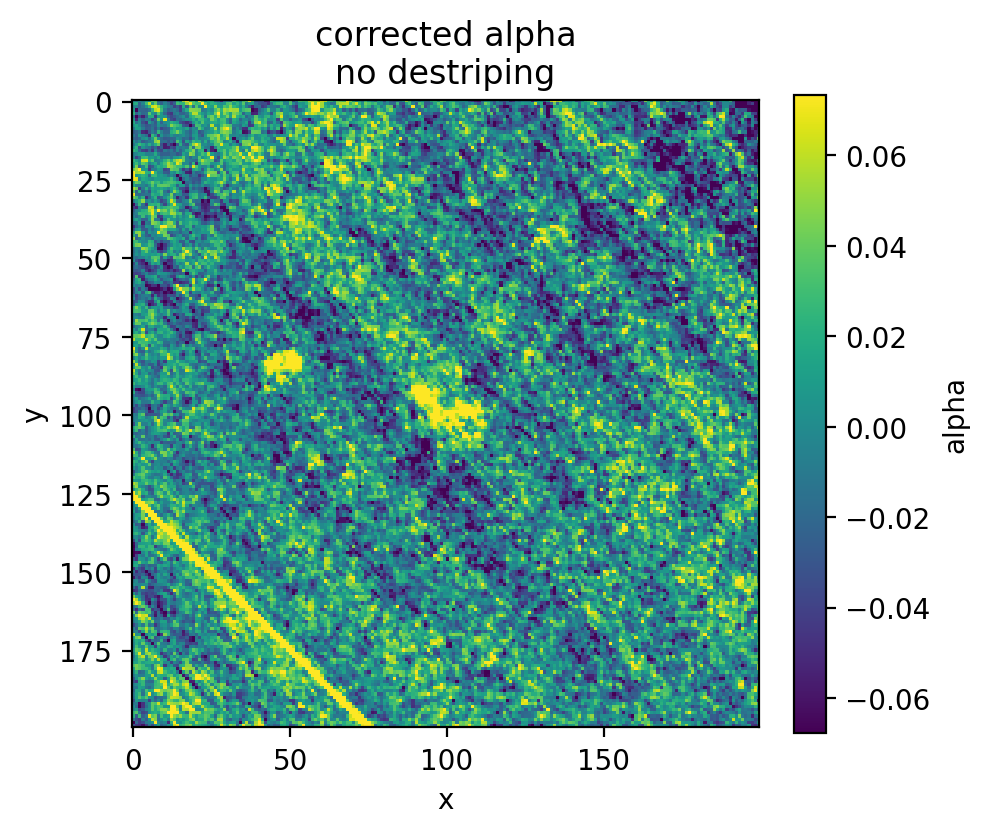
\includegraphics[width=\linewidth]{baseline_corrected_alpha.png}
    \caption{Baseline}
  \end{subfigure}
  \hfill
  \begin{subfigure}{0.24\textwidth}
    \centering
    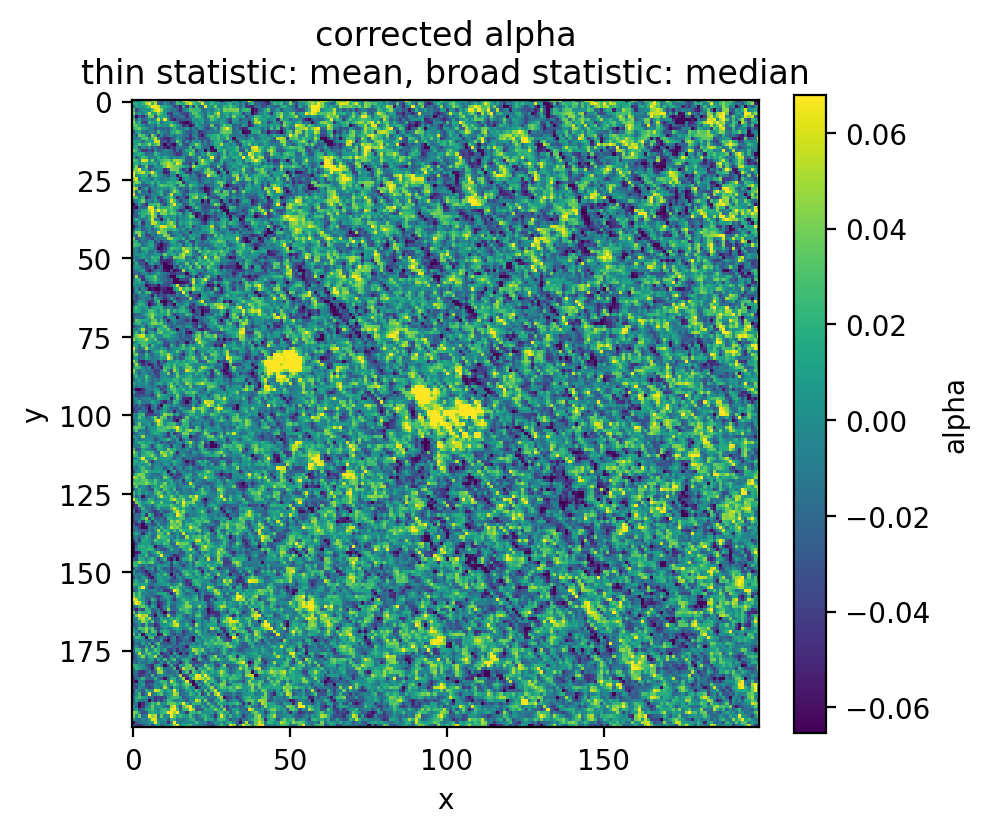
\includegraphics[width=\linewidth]{mean_corrected_alpha.png}
    \caption{Mean}
  \end{subfigure}
  \hfill
  \begin{subfigure}{0.24\textwidth}
    \centering
    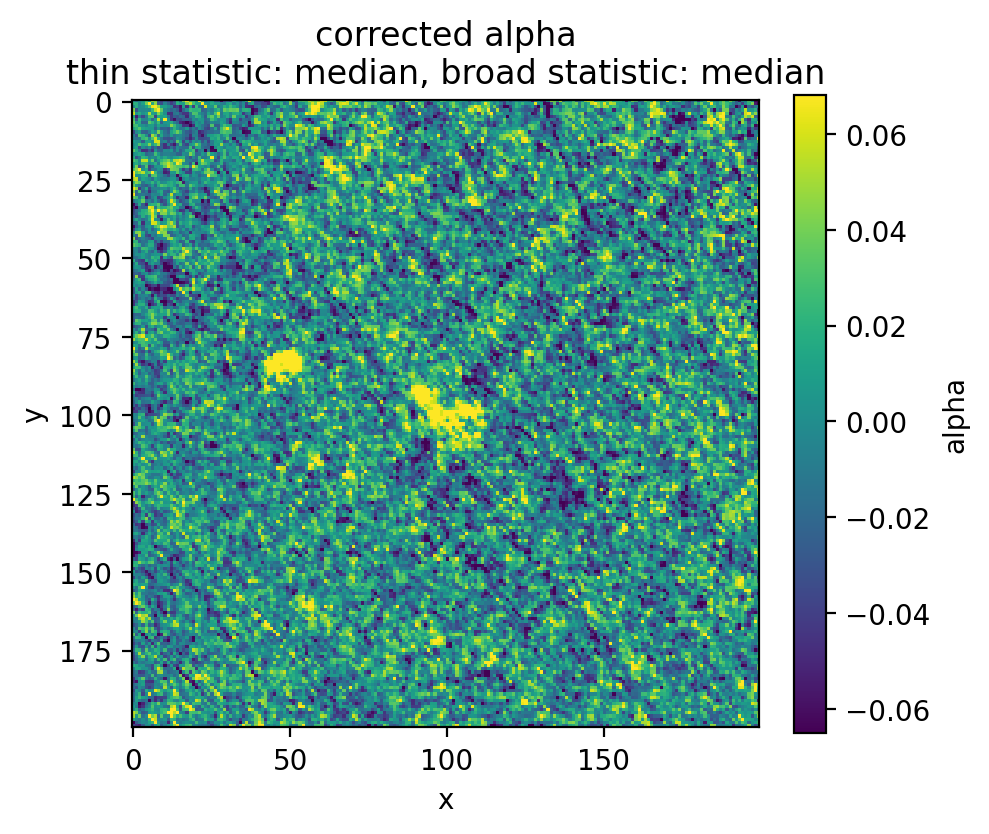
\includegraphics[width=\linewidth]{median_corrected_alpha.png}
    \caption{Median}
  \end{subfigure}
  \hfill
  \begin{subfigure}{0.24\textwidth}
    \centering
    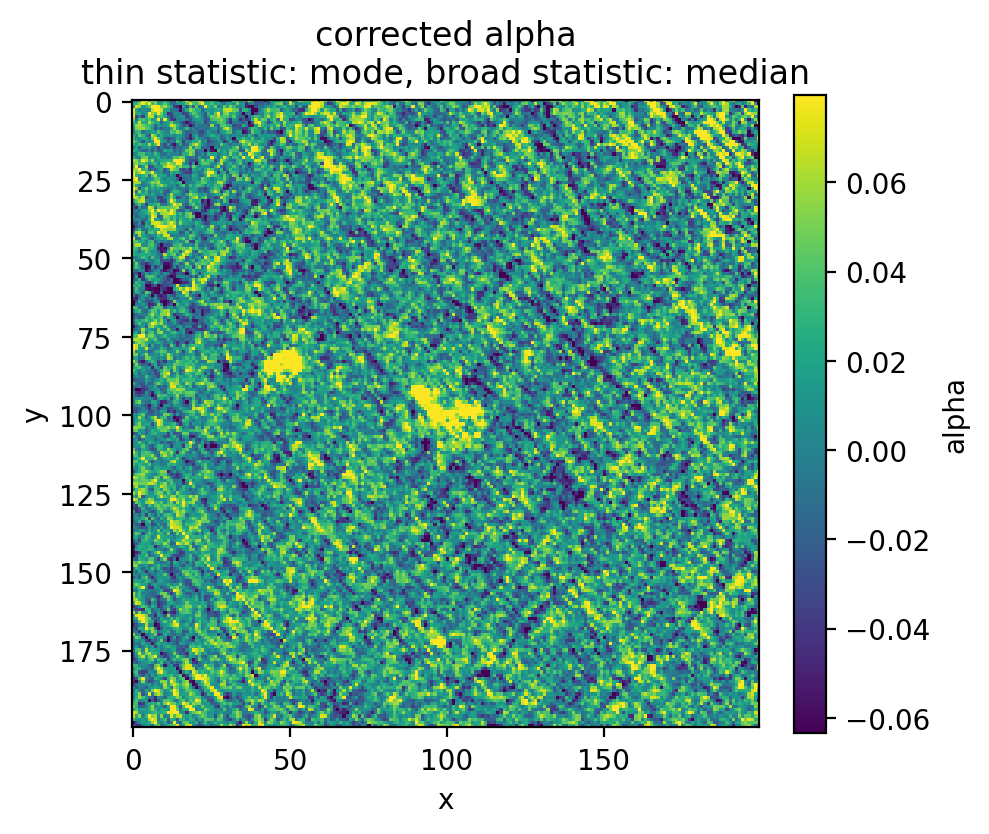
\includegraphics[width=\linewidth]{mode_corrected_alpha.png}
    \caption{Mode}
  \end{subfigure}
  \caption{Corrected-alpha comparison for different thin-line statistics. Broad-band cleanup used median in all non-baseline cases.}
  \label{fig:alpha_comparison}
\end{figure*}

\subsection{plume mask比較}
図\ref{fig:mask_comparison}に，統計量ごとのplume maskを示す．baselineでは左下の斜め線がmask上に残っている．meanではこの線状偽陽性が最も強く抑えられ，候補pixel数も最小になった．medianでは候補pixel数の削減はmeanより小さいが，alpha画像全体のRStdは最小であった．modeでは候補pixel数は減少したものの，RStd改善が小さく，補正後のalpha分布が安定しにくい結果となった．

\begin{figure*}[t]
  \centering
  \begin{subfigure}{0.24\textwidth}
    \centering
    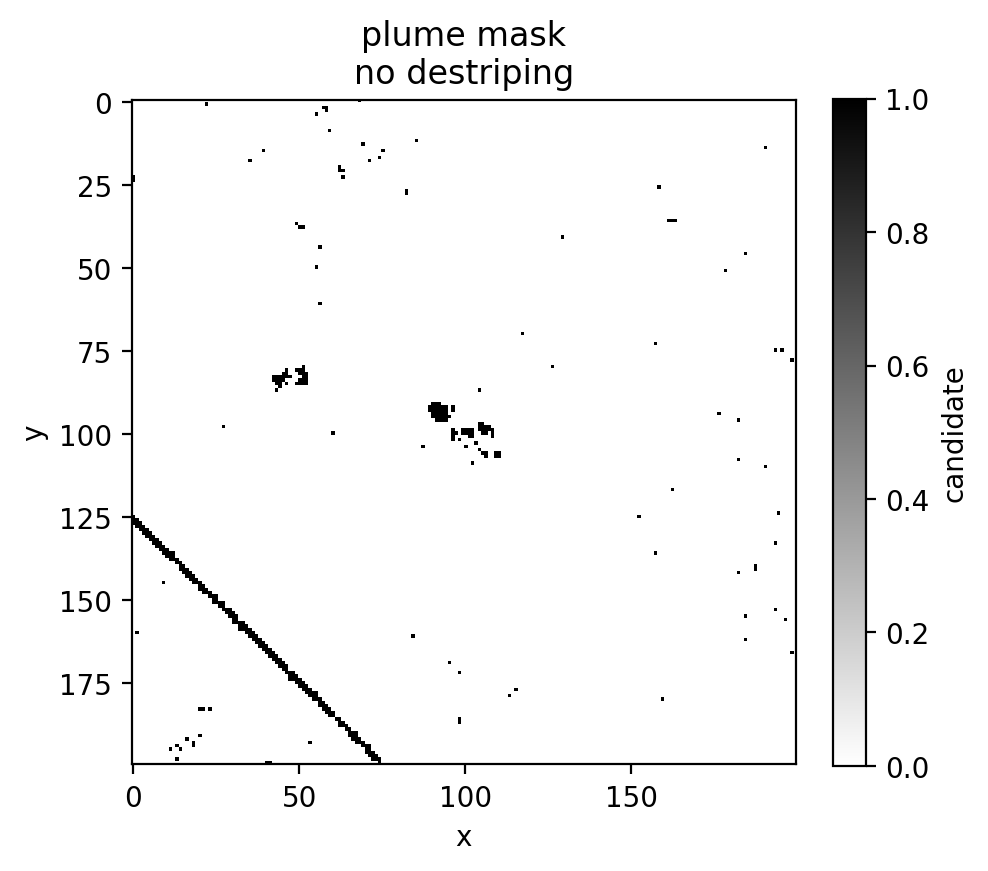
\includegraphics[width=\linewidth]{baseline_plume_mask.png}
    \caption{Baseline}
  \end{subfigure}
  \hfill
  \begin{subfigure}{0.24\textwidth}
    \centering
    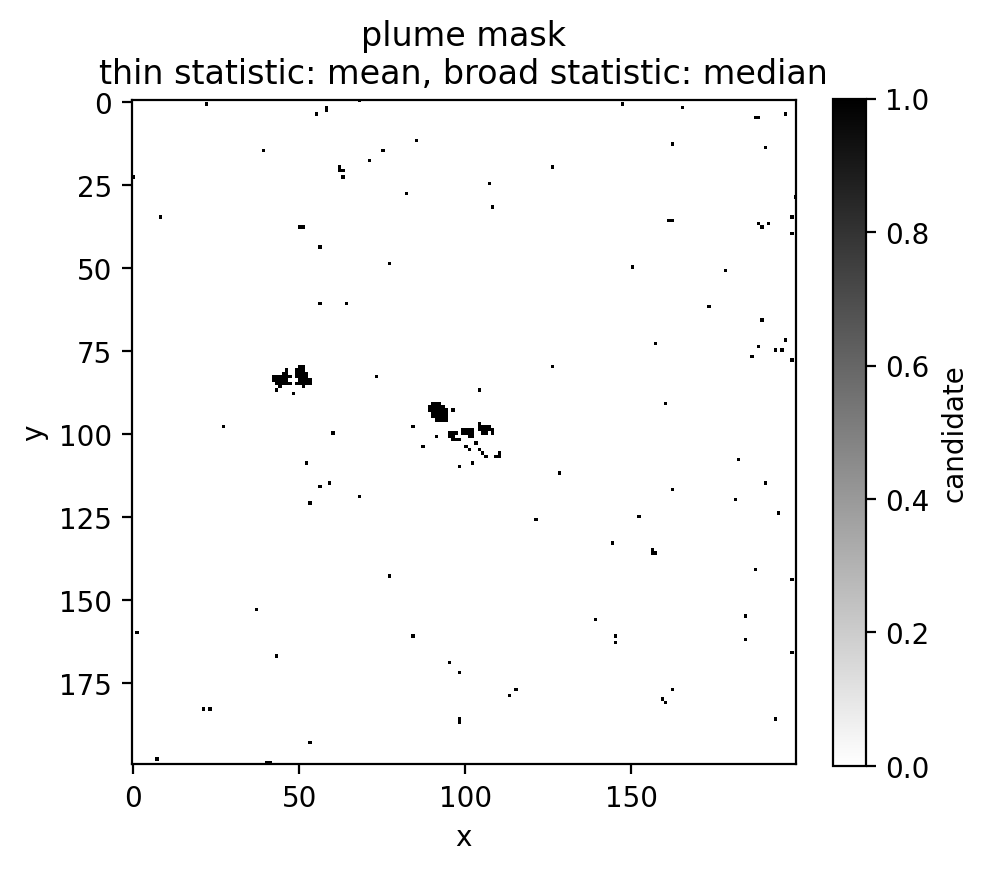
\includegraphics[width=\linewidth]{mean_plume.png}
    \caption{Mean}
  \end{subfigure}
  \hfill
  \begin{subfigure}{0.24\textwidth}
    \centering
    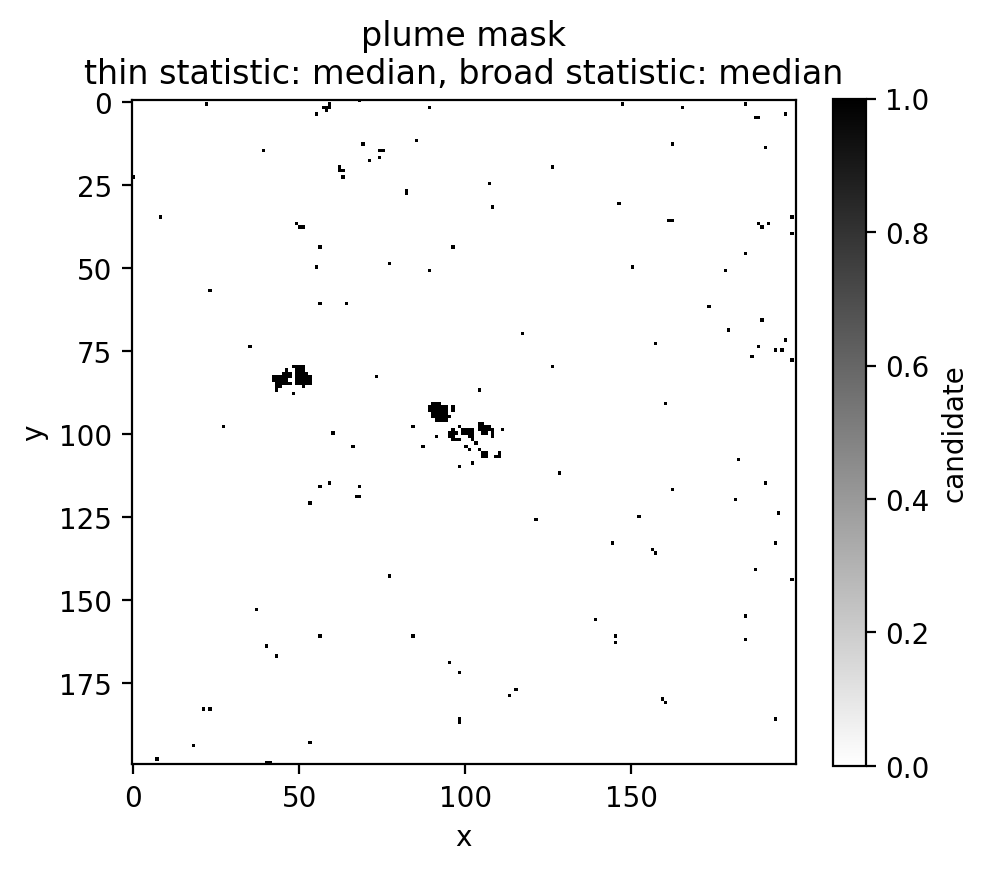
\includegraphics[width=\linewidth]{median_plume_mask.png}
    \caption{Median}
  \end{subfigure}
  \hfill
  \begin{subfigure}{0.24\textwidth}
    \centering
    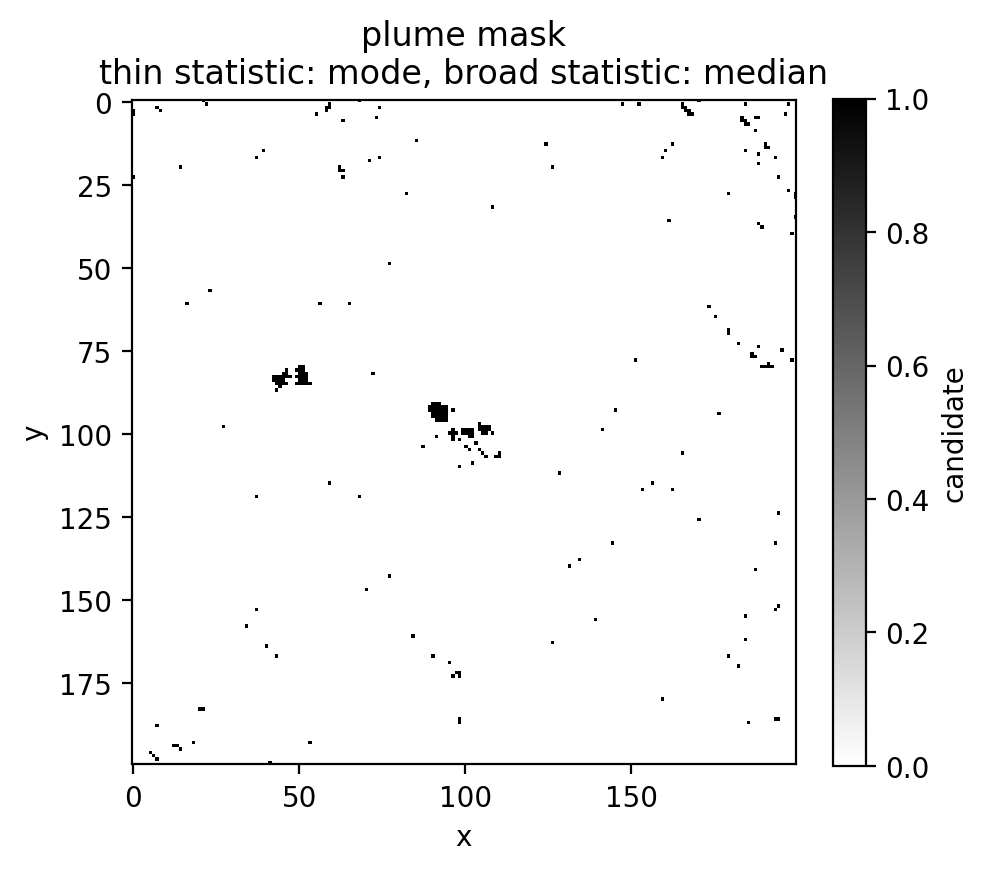
\includegraphics[width=\linewidth]{mode_plume_mask.png}
    \caption{Mode}
  \end{subfigure}
  \caption{Plume-mask comparison for different thin-line statistics. Mean reduced line-shaped false positives most strongly, whereas median provided the most stable alpha dispersion.}
  \label{fig:mask_comparison}
\end{figure*}

\subsection{定量比較}
表\ref{tab:result}と図\ref{fig:metric_comparison}に，baselineと各統計量の定量比較を示す．baselineではplume maskの候補pixel数は408，RStdは0.031263であった．meanでは候補pixel数が222まで減少し，45.6\%の削減となった．一方，medianではRStdが0.027978まで低下し，10.5\%の改善となった．modeは候補pixel数を263まで減少させたが，RStdは0.031175であり，baselineからの改善は小さかった．

この結果は，評価指標によって最適な統計量が変わることを示している．plume mask上の線状偽陽性を最優先で消すならmeanが有利である．alpha画像全体の安定性を重視するならmedianが有利である．本研究の用途では，plume mask上の偽陽性削減が重要であるためmeanに注目したが，最終的なメタン検出としては，スペクトル的な妥当性確認と組み合わせて判断する必要がある．

\begin{table}[t]
  \centering
  \caption{Quantitative comparison of line statistics for thin-line cleanup. Broad-band cleanup used median in all non-baseline cases.}
  \label{tab:result}
  \footnotesize
  \setlength{\tabcolsep}{3pt}
  \begin{tabular}{@{}lrrrr@{}}
    \toprule
    Method & Plume & Red. & RStd & RStd red.\\
    \midrule
    Baseline & 408 & 0.0\% & 0.031263 & 0.0\%\\
    Mean & \textbf{222} & \textbf{45.6\%} & 0.028486 & 8.9\%\\
    Median & 259 & 36.5\% & \textbf{0.027978} & \textbf{10.5\%}\\
    Mode & 263 & 35.5\% & 0.031175 & 0.3\%\\
    \bottomrule
  \end{tabular}
\end{table}

\begin{figure}[t]
  \centering
  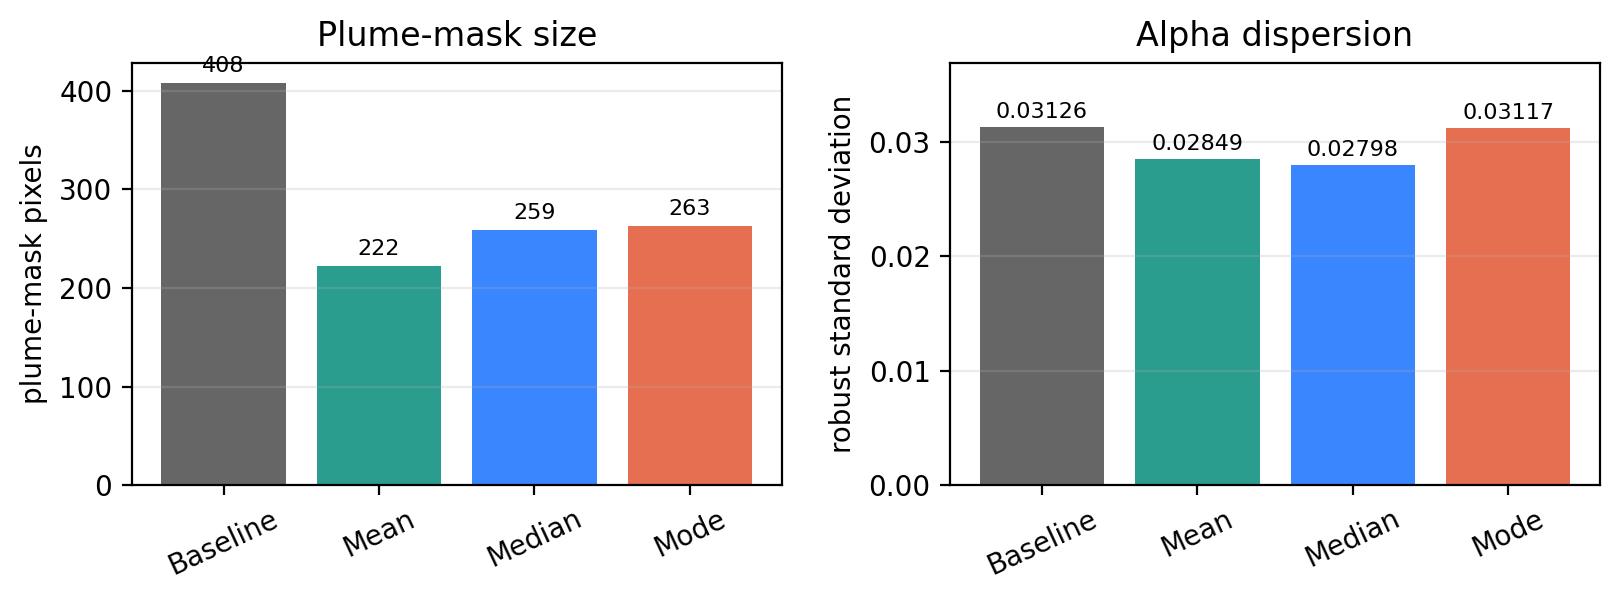
\includegraphics[width=\linewidth]{stat_metric_comparison.png}
  \caption{Metric comparison for baseline, mean, median, and mode. The left panel shows plume-mask pixels, and the right panel shows robust standard deviation of the alpha image.}
  \label{fig:metric_comparison}
\end{figure}

\section{選択pixelによるスペクトル確認}
\subsection{alpha値だけでは判断しにくい理由}
MF alphaはメタン吸収らしさを表す便利なスコアであるが，alpha値だけで実plumeと線状偽陽性を完全に区別することは難しい．線状ノイズがたまたまメタンテンプレートと相関するスペクトル偏差を持つ場合，MFはそれを高alphaとして出力する．したがって，高alpha pixelが実際にメタン吸収に対応しているかを確認するには，スペクトル残差や波長ごとのMF寄与を調べる必要がある．

図\ref{fig:selected_pixel_check}に，線上pixel，plume候補pixel，非plume control pixelを選び，RGB画像，MF alpha画像，fitted backgroundからの残差，波長別MF寄与を比較した結果を示す．線上pixelとplume候補pixelでは，alpha値だけでなく残差スペクトルの形やMF寄与の波長依存性が異なっている．特に，特定波長に鋭く寄与が出るpixelは，メタン吸収の広い構造というよりも，局所的なスペクトル異常やノイズの影響を受けている可能性がある．

\begin{figure*}[t]
  \centering
  \begin{subfigure}{0.40\textwidth}
    \centering
    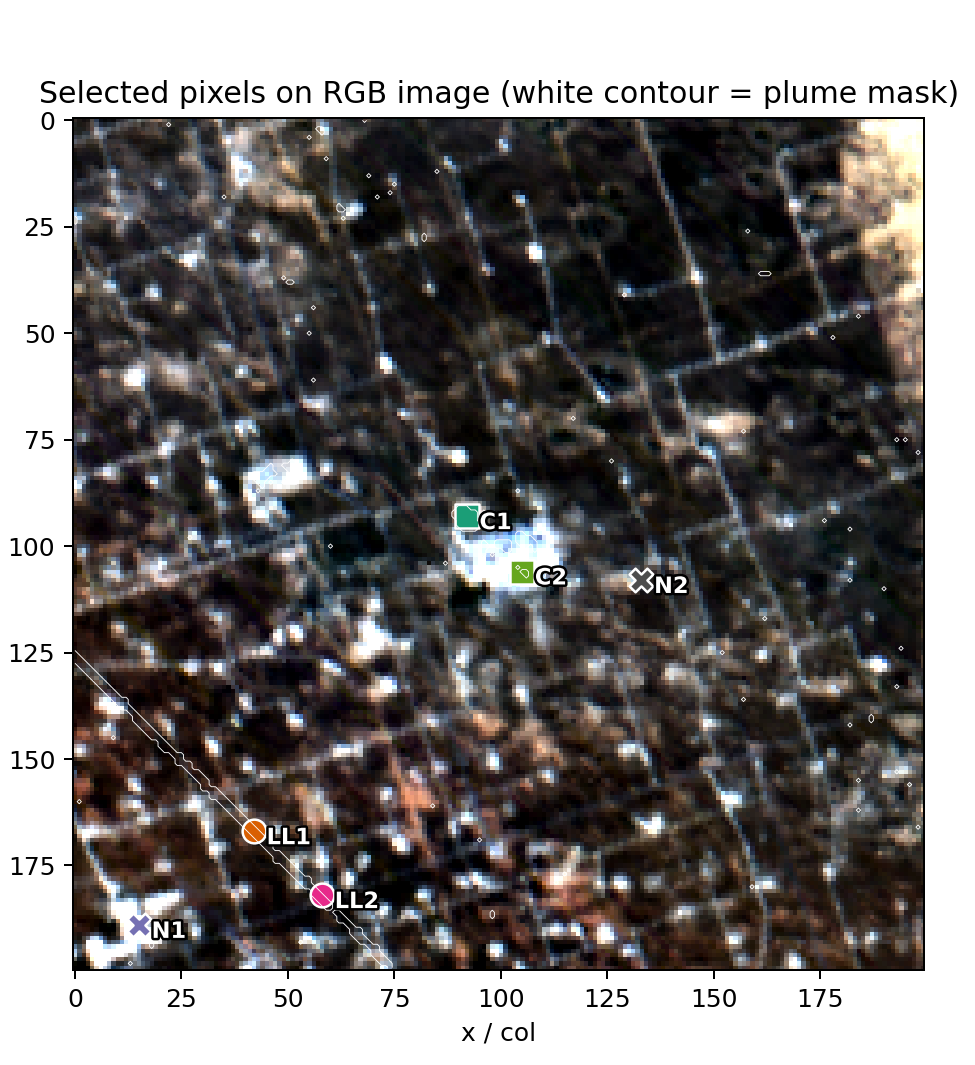
\includegraphics[width=\linewidth]{fig4_rgb_selected_pixels.png}
    \caption{Selected pixels on RGB}
  \end{subfigure}
  \hfill
  \begin{subfigure}{0.40\textwidth}
    \centering
    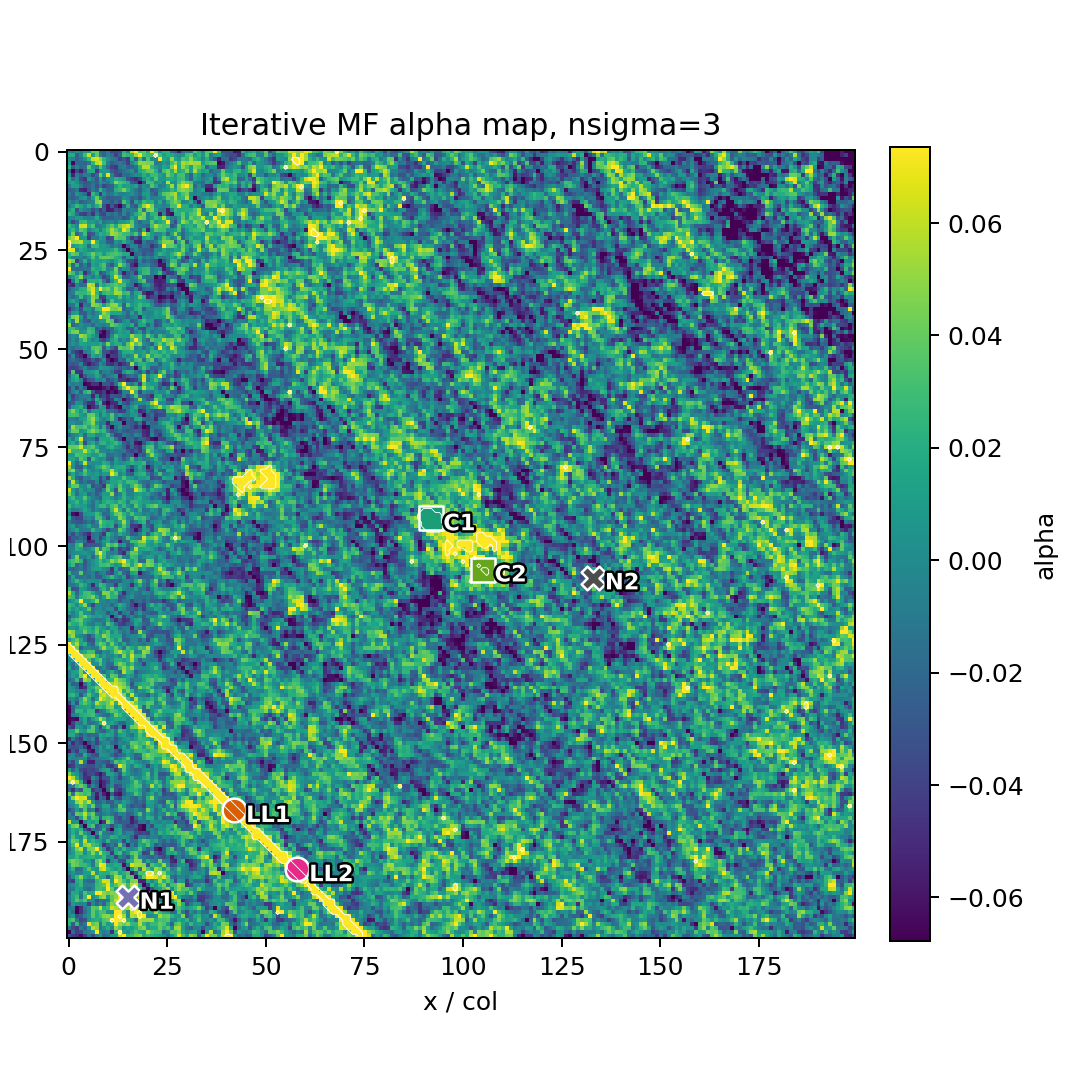
\includegraphics[width=\linewidth]{fig4_raw_alpha_selected_pixels.png}
    \caption{Selected pixels on MF alpha}
  \end{subfigure}

  \vspace{1mm}

  \begin{subfigure}{0.40\textwidth}
    \centering
    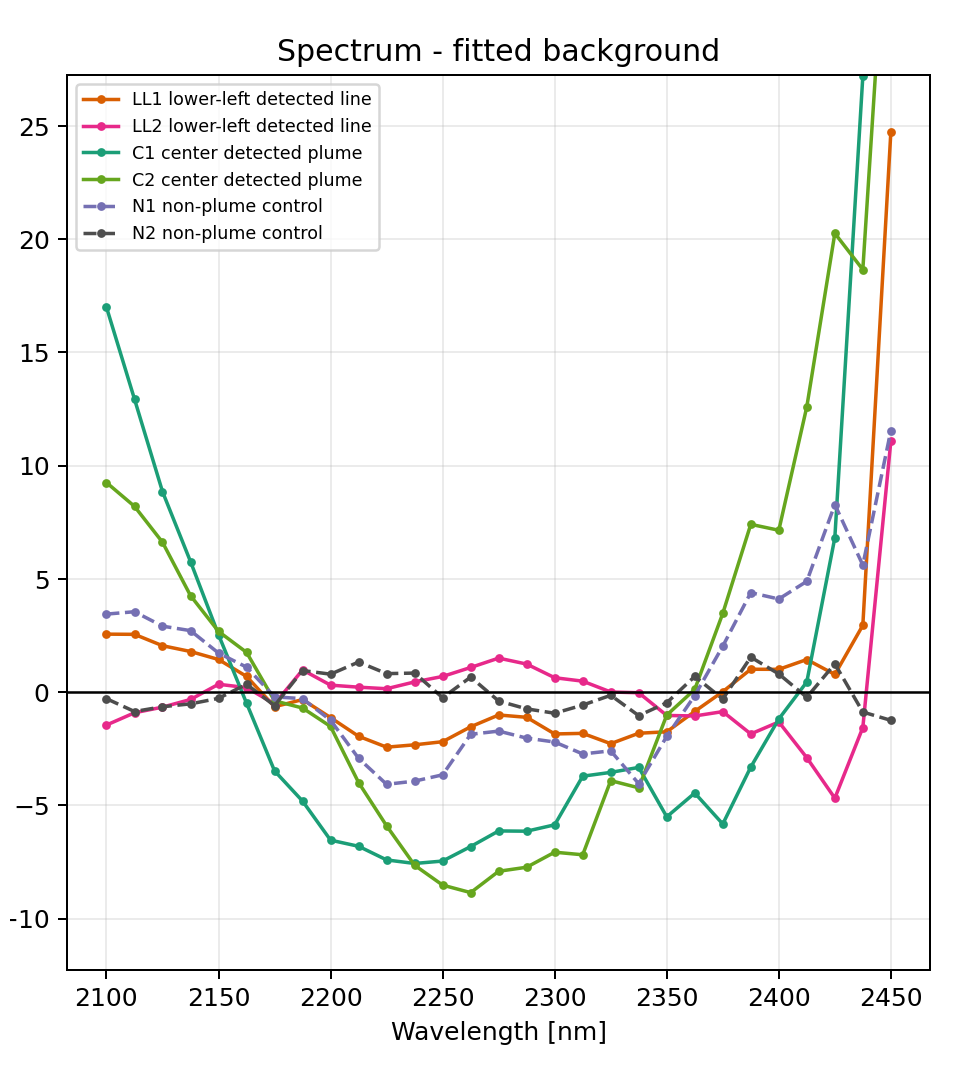
\includegraphics[width=\linewidth]{fig4_spectrum_fitted_background.png}
    \caption{Residual spectra}
  \end{subfigure}
  \hfill
  \begin{subfigure}{0.40\textwidth}
    \centering
    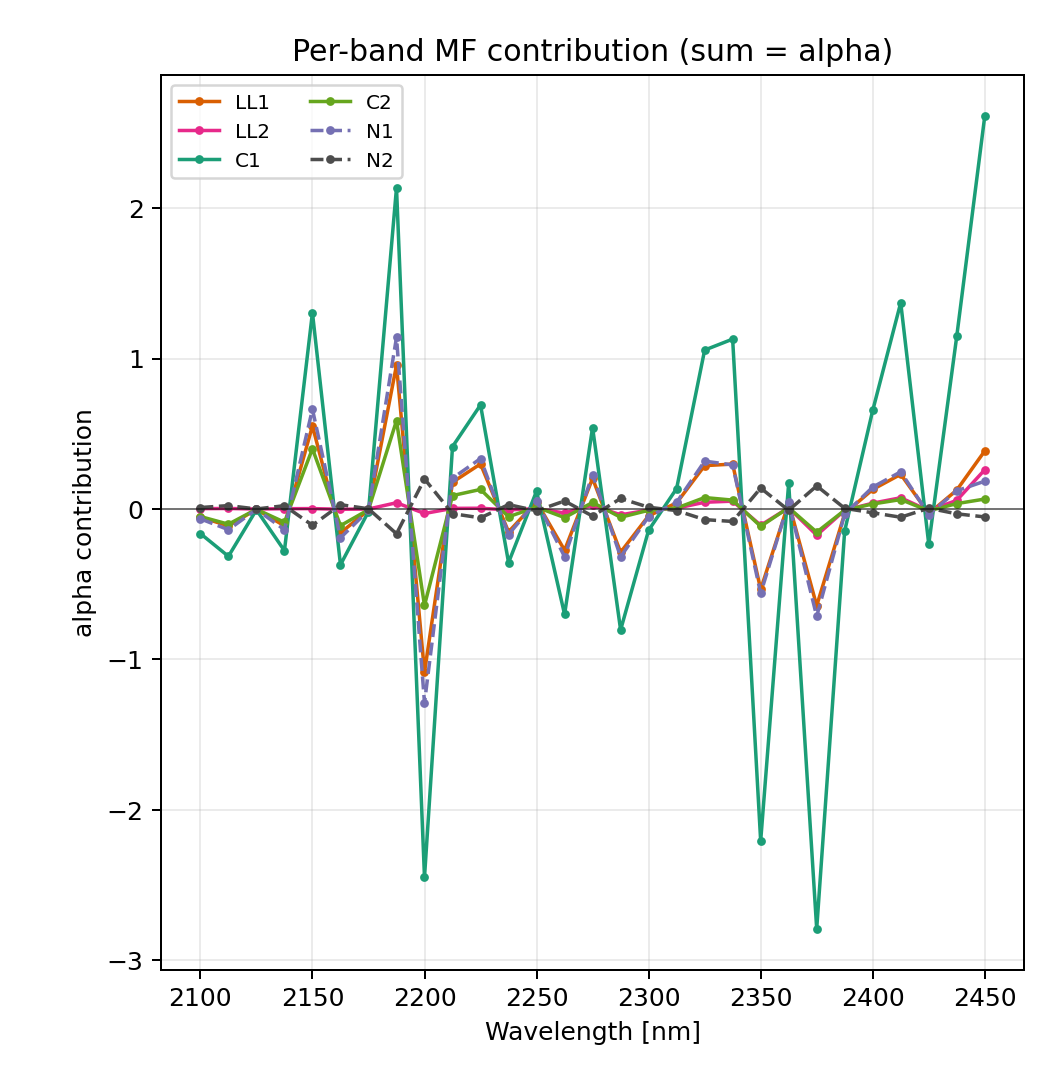
\includegraphics[width=\linewidth]{fig4_per_band_mf_contribution.png}
    \caption{Per-band MF contribution}
  \end{subfigure}
  \caption{Selected-pixel check of the iterative MF result. The panels compare line-artifact pixels, plume-candidate pixels, and non-plume control pixels on the RGB image, MF alpha map, fitted-background residual spectra, and per-band MF contributions.}
  \label{fig:selected_pixel_check}
\end{figure*}

\subsection{今後追加するとよい確認図}
本稿に入れた図に加えて，今後さらに有効な図として，波長--放射輝度スペクトルそのものの比較が挙げられる．現在の図\ref{fig:selected_pixel_check}では，fitted backgroundからの残差とMF寄与を示しているが，元の放射輝度スペクトル，背景スペクトル，メタン吸収テンプレートを同じ図に重ねると，非専門の聴衆にも「どの波長でメタンらしさを見ているか」が伝わりやすい．また，iterationごとのplume mask変化を並べる図があると，Iterative MFによって背景maskがどのように更新されるかを説明しやすい．

\section{考察}
\subsection{MFとdestripingの関係}
MFはスペクトル方向の検出器であり，destripingは画像空間上の補正である．一見すると別の処理に見えるが，本研究では両者が強く関係している．MFは背景平均と共分散に基づいてスペクトル的な偏差をalpha画像に変換する．もし画像空間上に線状の系統誤差があると，その誤差が特定のスペクトル方向に投影され，高alpha線として現れる可能性がある．したがって，alpha画像上でline groupごとのoffsetを補正することは，MF出力に残った空間的な系統誤差を取り除く処理と解釈できる．

ただし，destripingは後処理であり，メタン吸収そのものを物理的に推定しているわけではない．線状偽陽性を抑える効果はあるが，実plumeが同じ線方向に存在する場合，plume信号まで弱める可能性がある．このため，補正量の推定では，細い線と太いoffsetで高alpha除外の有無を変えた．また，最終的にはスペクトル確認により，補正後に残る候補がメタン吸収として妥当かを確認する必要がある．

\subsection{統計量選択の解釈}
mean，median，modeの比較から，統計量の選択は単なる実装上の違いではなく，何をノイズと見なすかに対応していることが分かった．meanはline group内の高alpha pixelを強く反映するため，細い高alpha線を消すには有効である．しかし，実plumeがgroup内に含まれる場合，補正量が大きくなりすぎる可能性がある．medianは外れ値に強く，画像全体のばらつき低下には有効であるが，細い線のようにgroup内の一部だけが大きくなる現象には鈍い場合がある．modeは分布の最頻値を使うため直感的には背景値を推定できそうだが，連続値画像ではbinningに敏感であり，本解析では安定しなかった．

\subsection{限界}
本研究の結果は，一つのHISUIシーンと200$\times$200 pixelのROIに基づく初期検討である．検出された傾きやbin幅は，このシーンの幾何やノイズ構造に依存している可能性がある．また，現在の評価はplume mask pixel数とRStdを中心としており，実際のメタン濃度や排出量の定量精度までは評価していない．さらに，destripingにより偽陽性が減る一方で，弱い実plumeが消える可能性もあるため，既知のplumeやシミュレーションデータを用いた検証が必要である．

\section{まとめと今後の課題}
本研究では，HISUI短波長赤外データに対するMFおよびIterative MFの出力に現れる線状ノイズを解析し，シーン全体から検出した線方向に沿ったdestripingをIterative MF内に組み込む方法を検討した．線状応答は，細い高alpha線と太い帯状offsetに分けて扱う必要があった．細い線には高alpha pixelの集中度に基づく傾き検出が有効であり，太いoffsetにはline group補正後のRStd低下を基準とする検出が有効であった．

thin-line cleanupの統計量比較では，meanがplume mask候補pixel数を最も大きく削減し，medianがalpha画像全体のRStdを最も低下させた．modeは候補pixel数を削減したものの，RStd改善が小さく，安定性に課題があった．選択pixelのスペクトル確認からは，線状偽陽性とplume候補では残差スペクトルや波長別MF寄与が異なることが確認された．

今後は，補正後に残るplume候補が実際のメタン吸収スペクトルに対応しているかを，放射輝度スペクトル，背景スペクトル，メタンテンプレートを直接比較して検証する必要がある．また，iterationごとの背景mask更新を可視化し，destripingが背景推定に与える影響を評価することも重要である．最終的には，後処理としてのdestripingだけでなく，背景推定やターゲットスペクトルの段階で線状ノイズに反応しにくいMFを構築することが課題である．

\begin{thebibliography}{9}
\small
\bibitem{mf}
C. C. Funk, J. Theiler, D. A. Roberts, and C. C. Borel, ``Clustering to improve matched filter detection of weak gas plumes in hyperspectral thermal imagery,'' IEEE Trans. Geosci. Remote Sens., vol. 39, no. 7, pp. 1410--1420, 2001, doi: 10.1109/36.934073.

\bibitem{foote2020}
M. D. Foote, P. E. Dennison, A. K. Thorpe, D. R. Thompson, S. Jongaramrungruang, C. Frankenberg, and S. C. Joshi, ``Fast and accurate retrieval of methane concentration from imaging spectrometer data using sparsity prior,'' IEEE Trans. Geosci. Remote Sens., vol. 58, no. 9, pp. 6480--6492, 2020, doi: 10.1109/TGRS.2020.2976888.

\bibitem{pei2023}
Z. Pei, G. Han, H. Mao, C. Chen, T. Shi, K. Yang, X. Ma, and W. Gong, ``Improving quantification of methane point source emissions from imaging spectroscopy,'' Remote Sens. Environ., vol. 295, 113652, 2023, doi: 10.1016/j.rse.2023.113652.

\bibitem{koga2011}
M. Koga and A. Iwasaki, ``Improving the measurement accuracy of three-dimensional topography changes using optical satellite stereo image data,'' IEEE Trans. Geosci. Remote Sens., vol. 49, no. 8, pp. 2918--2923, 2011, doi: 10.1109/TGRS.2011.2119398.

\bibitem{emit}
EMIT Science Team, ``Greenhouse gas point source mapping and related products,'' Algorithm Theoretical Basis Document, NASA/JPL, 2023.
\end{thebibliography}

\end{document}
